% ---------------------------------------------------------------------------
% Initial Situation
\begin{frame}
    \frametitle{Initial Situation}
    \centering
    \includegraphics[width=0.8\linewidth]{../assets/collage_sound_pollution.png}
\end{frame}
% ---------------------------------------------------------------------------

% ---------------------------------------------------------------------------
% Project Goals
\begin{frame}
    \frametitle{Project Goals}
    \begin{itemize}[<+->]
        \large
        \item Analyze Audio File
        \item Summarize findings in a PDF
        \item Easy to use
    \end{itemize}
\end{frame}
% ---------------------------------------------------------------------------

% Audio Files
\begin{frame}
    \frametitle{Audio Files}
    \centering
    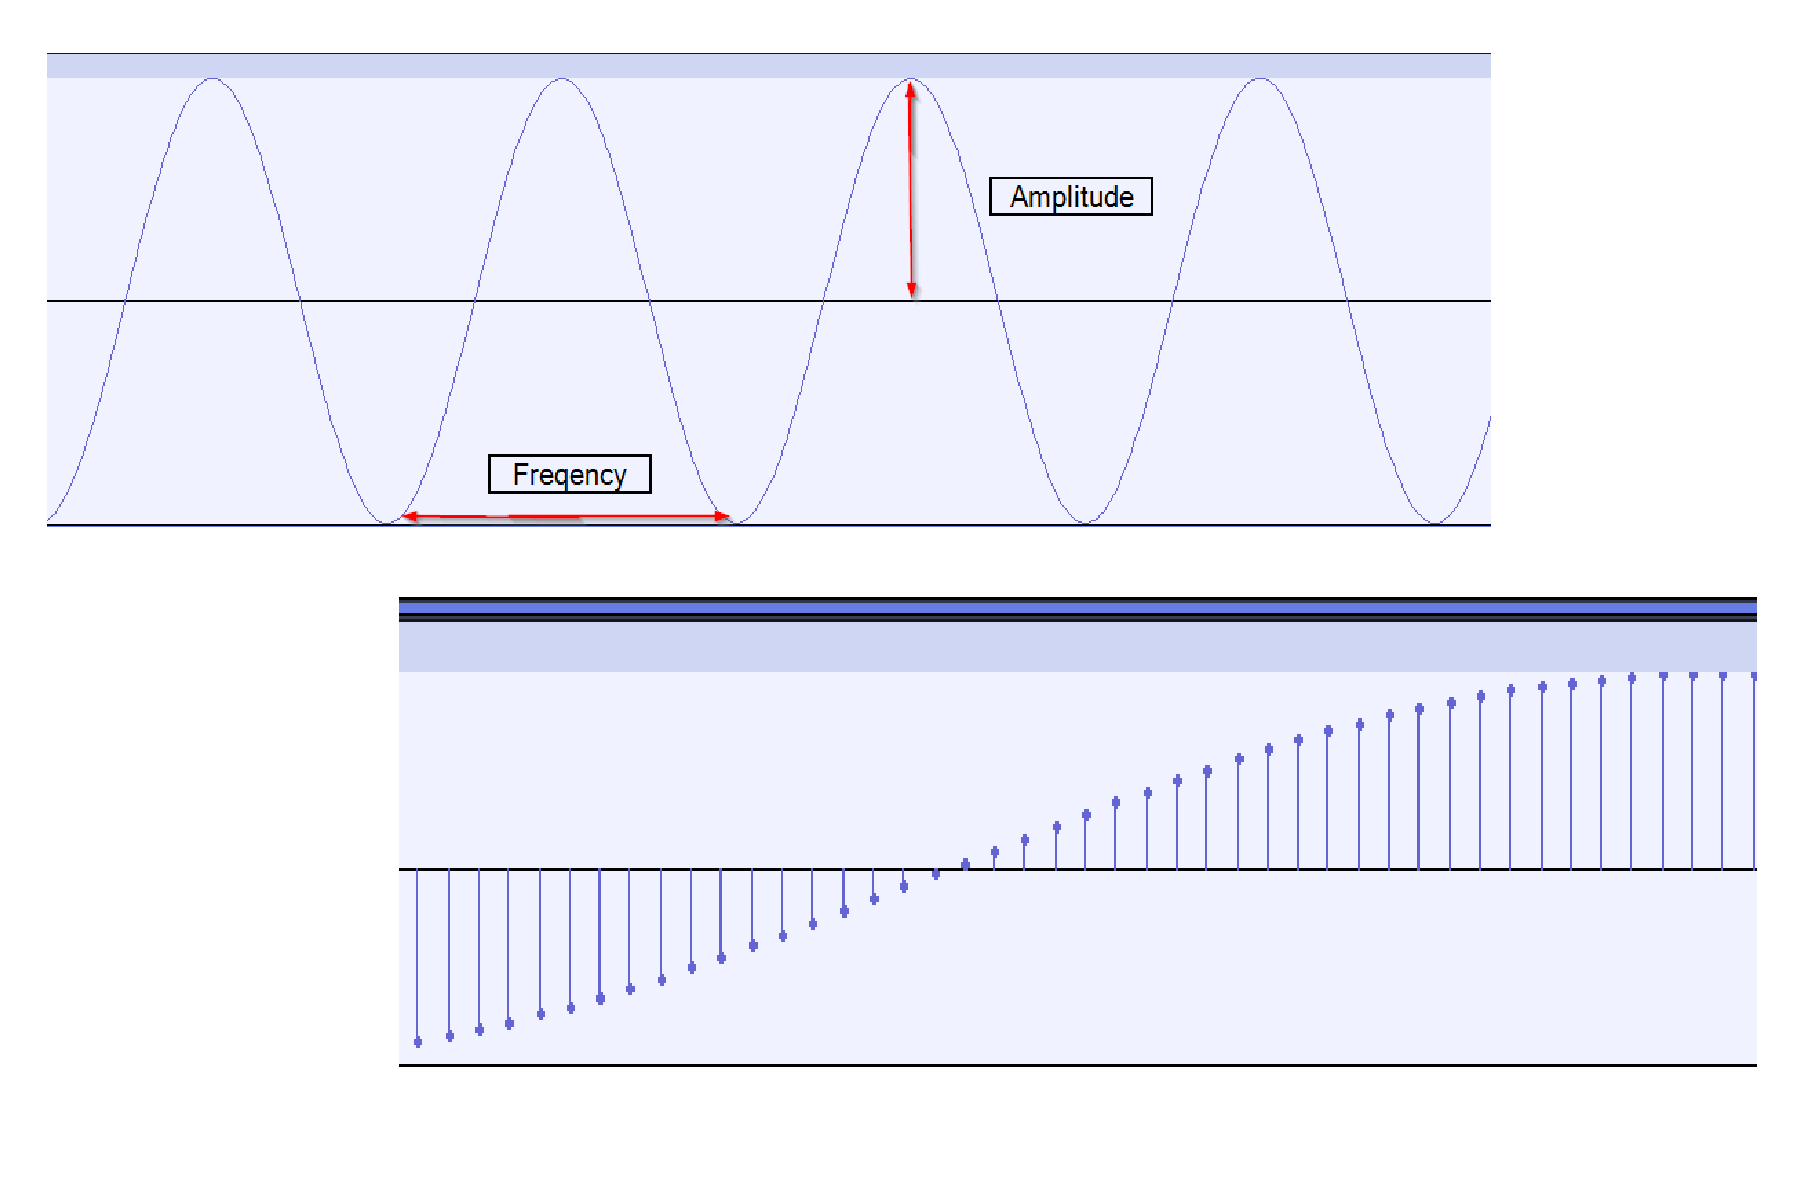
\includegraphics[width=0.8\linewidth]{../assets/audiofile_description.png}
\end{frame}
% ---------------------------------------------------------------------------

% Measuring the Sound Level
\begin{frame}
    \frametitle{Measuring the Sound Level}
    \centering
    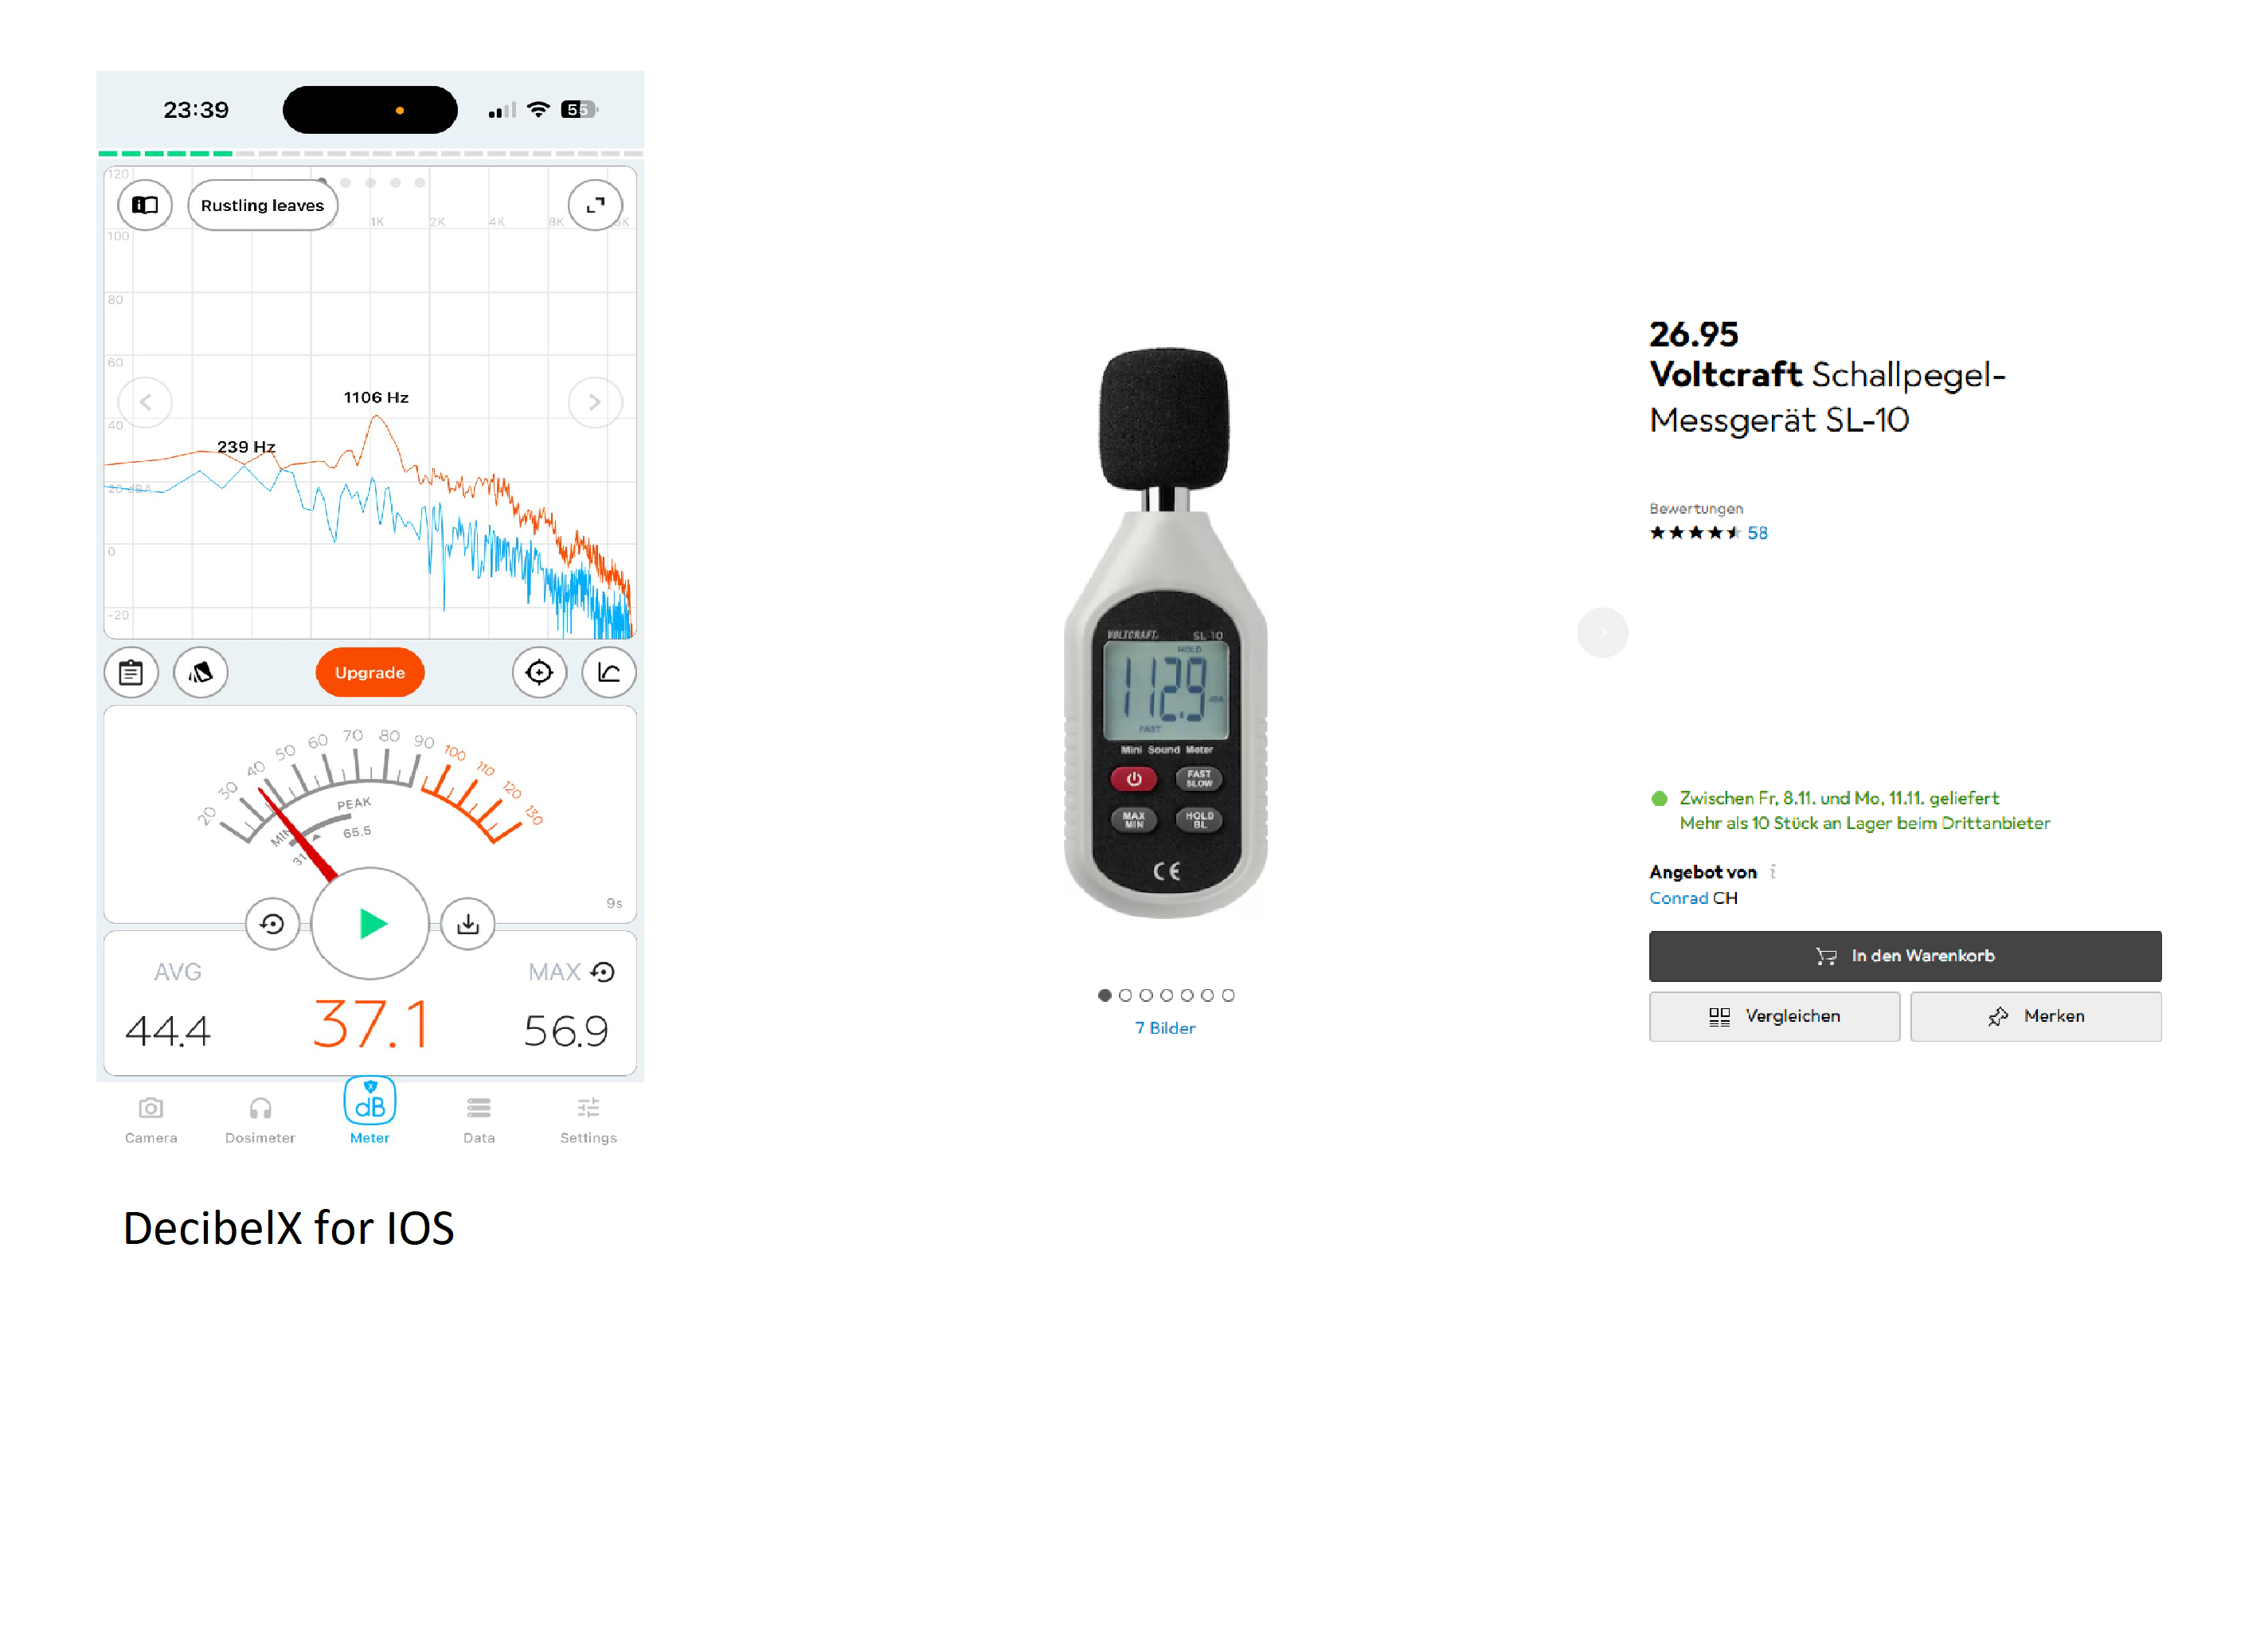
\includegraphics[width=0.8\linewidth]{../assets/measure_sound_level.png}
\end{frame}
% ---------------------------------------------------------------------------

% Requirements
\begin{frame}
    \frametitle{Requirements}
    \begin{itemize}[<+->]
        \large
        \item Take .wav file, threshold and additional reference values as input
        \item Analyze and Summarize 
        \begin{itemize}
            \large
            \item Metadata
            \item Plot
        \end{itemize}
        \item User should not need any Technical know-How
        \item Platform independent
        \item Multiple Languages
    \end{itemize}
\end{frame}
% ---------------------------------------------------------------------------